%%%%%%%%%%%%%%%%%%%%%%%%%%%%%%%%%%%%%%%%%%%%%%%%%%%%%%%%%%%%%%%%%%%%%%%%%%
 %																		%
 %	Plantilla Latex para presentación del proyecto de curso				%
 %	Programación de Aplicaciones para Internet y la Nube					%
 %																		%
 %	Creada por: Duván Pardo, Wilson López								%
 %																		%
 %	Versión: 0.2															%
 %	Dapardoc@gmail.com ; Wilrilo@gmail.com								%
 %																		% 
 %	Se requieren los archivos  plantilla.bbl								% 
 %	El directorio Imagenes que contiene: CECAD,DC, Elementos y RITA		%  
 %																		%
%%%%%%%%%%%%%%%%%%%%%%%%%%%%%%%%%%%%%%%%%%%%%%%%%%%%%%%%%%%%%%%%%%%%%%%%%%

\documentclass[10pt]{article}   			% Describe el tipo de documento, y el tamaño de la letra del texto

\usepackage[utf8]{inputenc}				% Define codificación para que permita caracteres latinos (acentos)
\usepackage[spanish,activeacute]{babel} 	% Paquete para poder escribir con tildes y otros caracteres especiales

\usepackage{vmargin}						% Código para margenes y formato de página
\setpapersize{A4}
\setmargins	{2.2cm}     					% margen izquierdo
			{1 cm}                 		% margen superior
			{16.5cm}               		% anchura del texto
			{23.42cm}             		% altura del texto
			{20pt}                		% altura de los encabezados
			{1.2cm}               		% espacio entre el texto y los encabezados
			{0pt}                		% altura del pie de página
			{2cm}                 		% espacio entre el texto y el pie de página

\usepackage{amsmath}						% paquete para expresiones matemáticas
\usepackage{amsfonts}					% paquete para escritura de ecuaciones 
\usepackage{amssymb}						% paquete para caracteres especiales para ecuaciones 

\usepackage{fancyhdr}					% Temas para encabezado y pie de pagina
\usepackage{fancyvrb}
\pagestyle{fancy} 

\pagenumbering{arabic} 					% Numeración de paginas {arabic roman}
\usepackage{hyperref}					% Para hipervinculos
\usepackage{graphicx}					% Para incluir imágenes
\usepackage{caption}						% Descripciones de las figuras
\usepackage{subcaption}					% Descripción varias imagenes en usa sola figura
\graphicspath{ {Imagenes/} }				% Directorio de imágenes esta capeta va donde esta el archivo tex


\usepackage{color, colortbl}				% Colores para tablas
\usepackage{listings}					% Para el código Fuente
\usepackage{xcolor}						% para color en codigos o listrings
\definecolor{limegreen}{RGB}{50,100,50}	% Definición de colores ejemplo verde en RGB
\definecolor{Red}{RGB}{220,120,120}		% se definen colores para la tabla en el cronograma pueden ser RGB 0-255 o rgb 0-1 cada componente
\definecolor{LightCyan}{rgb}{0.88,1,1}
\definecolor{azul}{RGB}{120,120,210}
\lstdefinestyle{base}{
	language=C,
	emptylines=1,
	breaklines=true,
	showspaces=fasle,
	showstringspaces=false,
	extendedchars=true,
	basicstyle=\ttfamily\color{black},
	moredelim=**[is][\color{limegreen}]{'}{'}, 	% Para este caso especial el caracter ' y & encierran
	moredelim=**[is][\color{blue}]{&}{&},		% un fragmento de código que quiere ser coloreado
}

\lstset{numbers=left, numberstyle=\tiny, stepnumber=2, numbersep=5pt}

%Aquí inicia el documento.
\begin{document}
	% Se define el Encabezado
	%clhead[]{Proyecto}
	\lhead[]{Programación de Aplicaciones para Internet y la Nube}
	\rhead[]{\textbf{2016-I}}
	\renewcommand{\headrulewidth}{0.5pt}

	\thispagestyle{empty}						% La primera página no lleva estilo (sin encabezado)
	\begin{center}
		\large {Programación de Aplicaciones para Internet y la Nube
			\hspace{5 cm}\textbf{2016-I}}
		\bigskip  
		\textbf{
			\LARGE{\\SENSORES INALÁMBRICOS E INTERNET DE LAS COSAS PARA DETECTAR CUELLOS DE BOTELLA}}\\								% Nombre del proyecto
	\end{center}	
	\begin{flushright}	
		\bigskip	
		Autor: \textbf{Yeny Katherine Muñoz Nuñez}			% Nombre del estudiante
	\end{flushright} 

	\textbf{Palabras clave}: Iaas, Saas, Paas, Cloud, Bottleneck		
	
\section{Introducción}

La visión de sistemas informáticos, presentes en todas partes, exige un cambio de modelo para integrar en nuestro entorno la potencia de cálculo, en lugar de tenerla concentrada en ordenadores de sobremesa o portátiles. Esta amplia visión del futuro ha impulsado varios campos de investigación poco definidos, entre ellos las redes de sensores inalámbricos.\\

Un sistema WSN (Wireless Sensor Network) de sensores inalámbricos es una red con numerosos dispositivos distribuidos espacialmente, que utilizan sensores para controlar diversas condiciones en distintos puntos, entre ellas la temperatura, el sonido, la vibración, la presión y movimiento o los contaminantes. Los dispositivos son unidades autónomas que constan de un microcontrolador, una fuente de energía (casi siempre una batería), un radiotransceptor y un elemento sensor.\\

Para el presente trabajo se busca investigar nuevas soluciones para la automatización industrial. Es muy importante mencionar que, al realizar la planeación de la producción, se tengan en cuenta aquellos \textit{cuellos de botella} que existen en el proceso para que así, los recursos que no son cuello de botella y no funcionen al 100 por ciento de su capacidad sean programados con respecto a los que si son. De esta manera se producirá sólo lo que puedan absorber los cuellos de botella reasignando la carga de trabajo de las máquinas que están sobrecargadas a las que tiene capacidad disponible.\\

\begin{figure}[ht] 
	\centering
		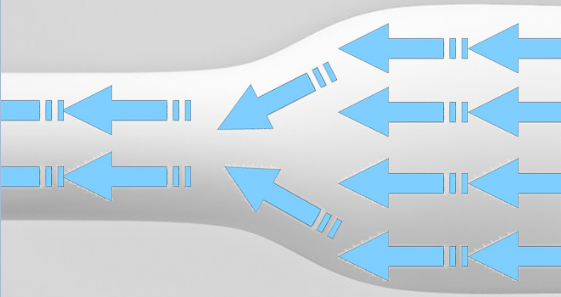
\includegraphics[scale=0.3]{CUELLOBOTELLA}   
	\caption{Representación gráfica de un cuello de botella [8.1]} \label{fig:CUELLO}
\end{figure}
		
\section{Descripción del proyecto}

La Teoría de las Restricciones o de Cuellos de Botella está basada en el simple hecho de que los procesos de cualquier ámbito, solo se mueven a la velocidad del paso más lento. La manera de balancear el proceso es utilizar un acelerador en este paso y lograr que trabaje hasta el límite de su capacidad para acelerar el proceso completo, estos factores limitantes se denominan restricciones, embudos o cuellos de botella. \\

Por supuesto las restricciones pueden ser un individuo, un equipo, la pieza de un aparato, una política local, o la ausencia de alguna herramienta o pieza de algún aparato. Por regla general en toda empresa hay, por lo menos, una restricción pues si así no fuera, generaría ganancias ilimitadas. Siendo las restricciones factores que bloquean a la empresa en la obtención de mayores ganancias, toda gestión gerencial que apunte a ese objetivo debe focalizarse sobre las restricciones.\\

Teniendo en cuenta las necesidades en este campo, se espera diseñar un modelo predictivo por medio del cual se detecten los cuellos de botella en un proceso industrial, haciendo uso de una red de sensores inalámbrico e internet de las cosas.

\begin{figure}[ht] 
	\centering
		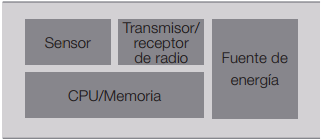
\includegraphics[scale=0.7]{SENSOR}   
	\caption{Dispositivo autónomo de una red de sensores inalámbricos [Aakvaag, 2006]} \label{fig:SENSOR}
\end{figure}

El proyecto se divide en los siguientes componentes:
		
\begin{itemize}
	\item \textbf{Adquisición de datos:} los datos se simularon por medio de un programa asociacdo a Visual Studio denominado Process Simulator. ProModel Solutions  propone establecer un modelo de su sistema en una herramienta de simulación 3D.
Los cuellos de botella serán detectados a través de los análisis estadísticas de los resultados pero también visualizados a través de la animación. Esta última etapa permite darse cuenta del impacto de las acumulaciones sobre el sistema.

\begin{figure}[ht] 
	\centering
		
\includegraphics[scale=0.7]{pcs2014}   
	\caption{Pantalla intro de Process Simulator 2014 [8.2]} \label{fig:pcs2014}
\end{figure}
		
	\item \textbf{Visualización de los datos en la nube:} se plantea subir los datos a el servidor de freeboard.io. Estamos ante un panel web sencillo que muestra la información de los diferentes dispositivos que tengas conectados en tiempo real.

\begin{figure}[ht] 
	\centering
		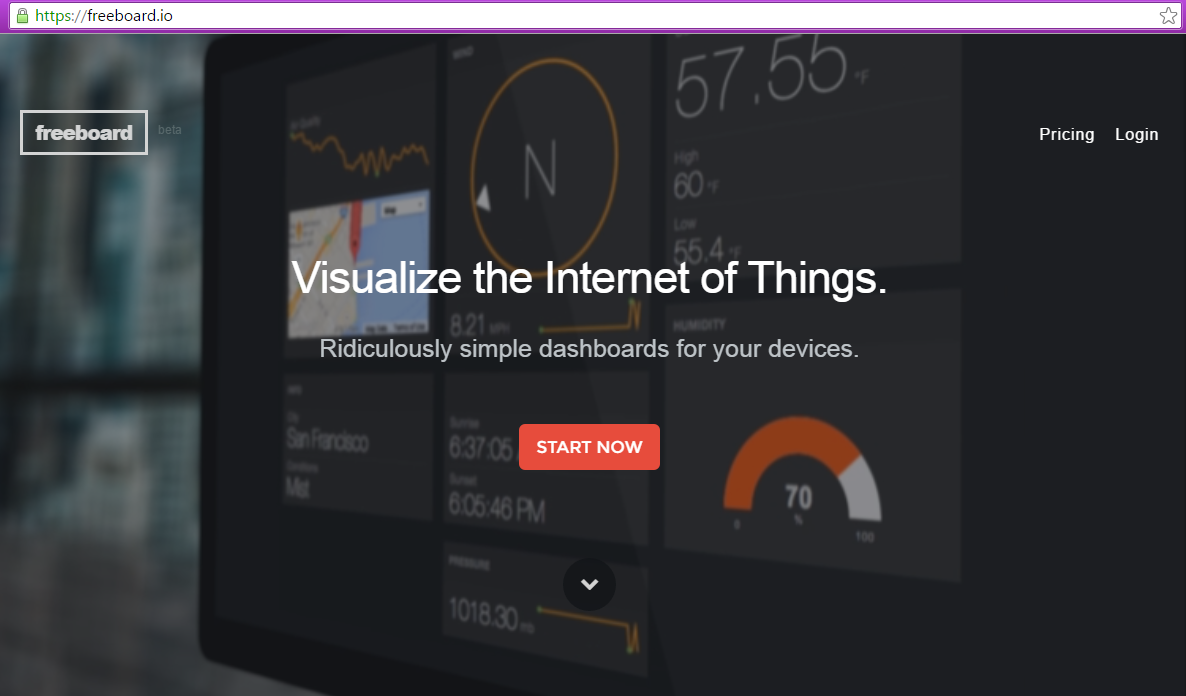
\includegraphics[scale=0.25]{freeboard}   
	\caption{Pantalla intro de freeboard.io [8.3]} \label{fig:freeboard}
\end{figure}
		
\end{itemize}
		

\newpage 

\section{Aplicaciones en la nube}

Cuando se hace referencia a desarrollar aplicaciones en la nube tenemos que definir de qué manera se va a implementar, ya que dentro del concepto nube existen distintas formas de hacerlo que permiten una mayor flexibilidad, agilidad y sencillez a la hora de desplegar aplicaciones o mantenerlas en operación. Entre estas distintas formas que puede adoptar la nube se encuentran:

\begin{itemize}
	\item Software Como Servicio (SaaS)
	\item Plataformas como Servicio (PaaS)
	\item Infraestructura como Servicio (IaaS)
\end{itemize}

\subsection{Software como Servicio (SaaS)}

El concepto de SaaS ha existido desde hace mucho tiempo, pero quizás en estos  últimos años se ha definido claramente a que se refiere. Básicamente se trata de cualquier servicio basado en la web.\\
	En este tipo de servicios se accede normalmente a través del navegador sin atender al software. Todo el desarrollo, mantenimiento, actualizaciones, copias de seguridad es responsabilidad del proveedor [Ohri, 2014]. En este se tiene poco control, el usuario se ubica en la parte más arriba de la capa del servicio. Si el servicio se cae es responsabilidad de proveedor hacer que vuelva a funcionar. \\
Ejemplos populares de Saas son Google Docs, Salesforce, Dropbox, Gmail. 
	
\subsection{Plataformas como Servicio (PaaS)}

PaaS es el punto donde los desarrolladores empiezan a desarrollar sus propias aplicaciones que se ejecutan en la nube. En este caso la única preocupación es la construcción de la aplicación, ya que la infraestructura la da la plataforma.\\
Es un modelo que reduce bastante la complejidad a la hora de desplegar y mantener aplicaciones ya que las soluciones PaaS gestionan automáticamente la escalabilidad usando más recursos si fuera necesario. Los desarrolladores aun así tienen que preocuparse de que sus aplicaciones estén lo mejor optimizadas posibles para consumir menos recursos posibles (número de peticiones, escrituras en disco, espacio requerido, tiempo de proceso, etc.).\\
Ejemplos populares son Google App Engine que permite desarrollar aplicaciones en Java o Python desplegándolas en la infraestructura que provee Google, cosa que también hace Heroku con Rails y Django.

\subsection{ Infraestructura como Servicio (IaaS)}

Con IaaS se tiene más control que con PaaS, aunque a cambio de eso el desarrollador tendrá que encargarse de la gestión de la infraestructura. \\
El ejemplo perfecto es el proporcionado por Amazon Web Service (AWS) que provee una serie de servicios como EC2 que permite manejar máquinas virtuales en la nube o S3 para usar como almacenamiento. Es posible elegir qué tipo de instancias se quieren usar Linux o Windows, así como la capacidad de memoria o procesador de cada una de las maquinas.\\
Además de AWS se encuentran plataformas como Rackspace Cloud o vCloud de VMWare.

\newpage		
\section{Desarrollo del Proyecto}

\subsection{Proceso de producción}

Se ejecuta en ciclos de ejecución diarios que se denominan día de producción. El día de producción es un plazo de 24 horas, pero no tiene que ajustarse a un día del calendario real. Podría existir desplazamiento. Por ejemplo, el día de producción por omisión se ejecuta desde las 06:00 hasta las 05:59 del día siguiente. Al inicio de cada día de producción, ejecuta un programa que selecciona las secuencias de trabajos que han de ejecutarse ese día de las bases de datos que se encuentran en el gestor de dominio maestro. A continuación, otro programa incluye las planificaciones no completas del día de producción anterior en la producción del día en curso y registra todas las estadísticas del día anterior en un archivo archivador.\\ \\
Toda la información que se necesita para ese día de producción se incluye en una base de datos de control de la producción. Durante el día de producción, la base de datos de control de la producción se actualiza continuamente para reflejar el trabajo que debe realizarse, el trabajo que está procesándose y el trabajo que se ha completado. Se envía una copia del archivo a todos los gestores de dominio subordinados y a todos los agentes tolerantes a errores del mismo dominio. Los gestores de dominio subordinados distribuyen su copia a todos los agentes tolerantes a errores de su dominio y a todos los gestores de dominio que son subordinados de éstos, y así sucesivamente hasta llegar al último elemento. Esto permite que los agentes tolerantes a errores de toda la red puedan seguir procesándose, incluso si se pierde la conexión de red con su gestor de dominio. Desde Simulation Porperties, el operador puede ver y realizar cambios en la producción del día aplicando los cambios en el archivo.\\ \\
Los procesos supervisan la base de datos de control de la producción y realizan llamadas al sistema operativo para iniciar trabajos en función de las necesidades. El sistema operativo ejecuta el trabajo y, posteriormente, informa acerca de si el trabajo se ha completado satisfactoriamente o no. Esta información se entra en la base de datos de control de la producción para indicar el estado del trabajo.

\subsection{Simulación de cadena de suministro y proceso de producción}

\begin{figure}[ht] 
	\centering
		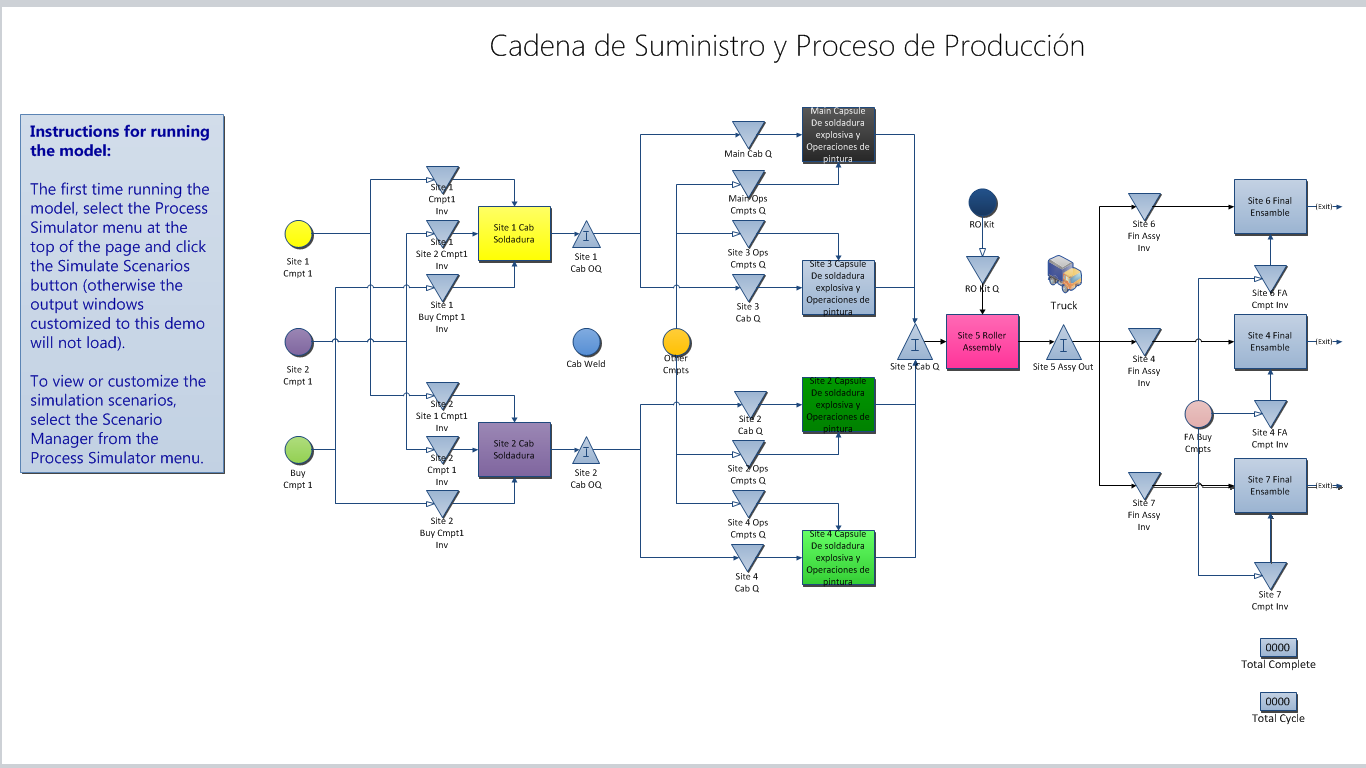
\includegraphics[scale=0.45]{procesodeproduccion}   
	\caption{ \href{https://youtu.be/TfvSbhoqySw}{Esquema del proceso de producción a simular}} \label{fig:procesodeproduccion}
\end{figure}

\newpage

\section{Resultados}

Resultado esperado la idea es que se den cuenta que programamos para Internet y la nube que se entiende Internet por internet de la nube, si es visualización de  plataformas o software para servicios, se tiene que trabajar en cecad pero también es importante llevarlo a la nube pública Amazon, Azure entre otras.

\begin{figure}[ht]
\centering
\begin{subfigure}[b]{0.45\textwidth}  		% el nunero se utiliza para cambiar la escala de la imagne
	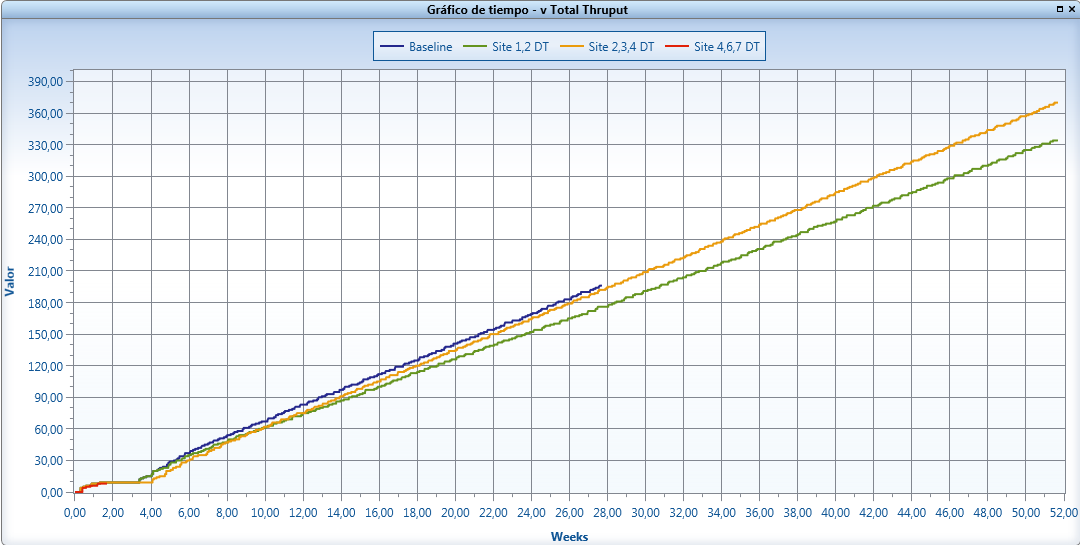
\includegraphics[width=\textwidth]{TIEMPO}
	\caption{Gráfica de Tiempo}
	\label{fig:TIEMPO}
\end{subfigure}
\begin{subfigure}[b]{0.4\textwidth}		 	% el nunero se utiliza para cambiar la escala de la imagne
	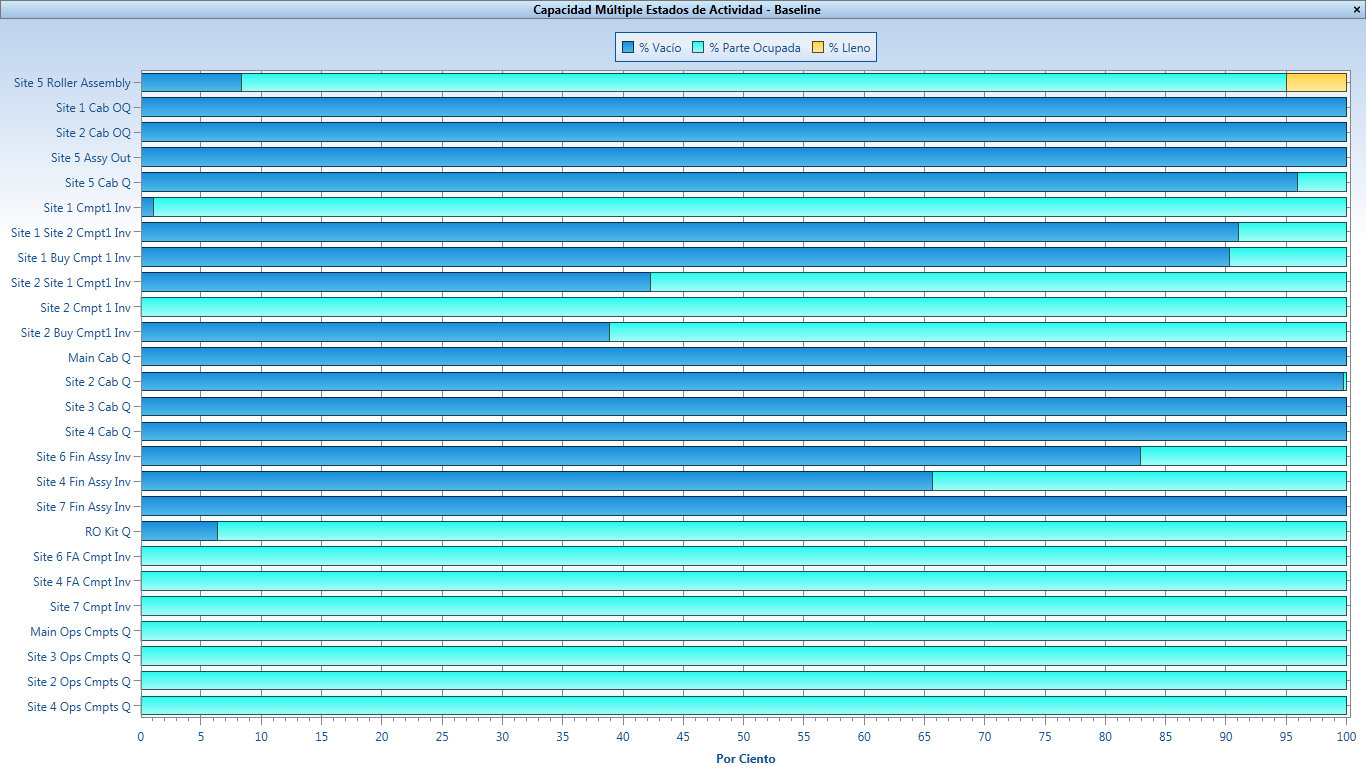
\includegraphics[width=\textwidth]{ACTIVIDAD}
	\caption{Estados de Actividad}
	\label{fig:ACTIVIDAD}
\end{subfigure}
\begin{subfigure}[b]{0.74\textwidth}		 	% el nunero se utiliza para cambiar la escala de la imagne
	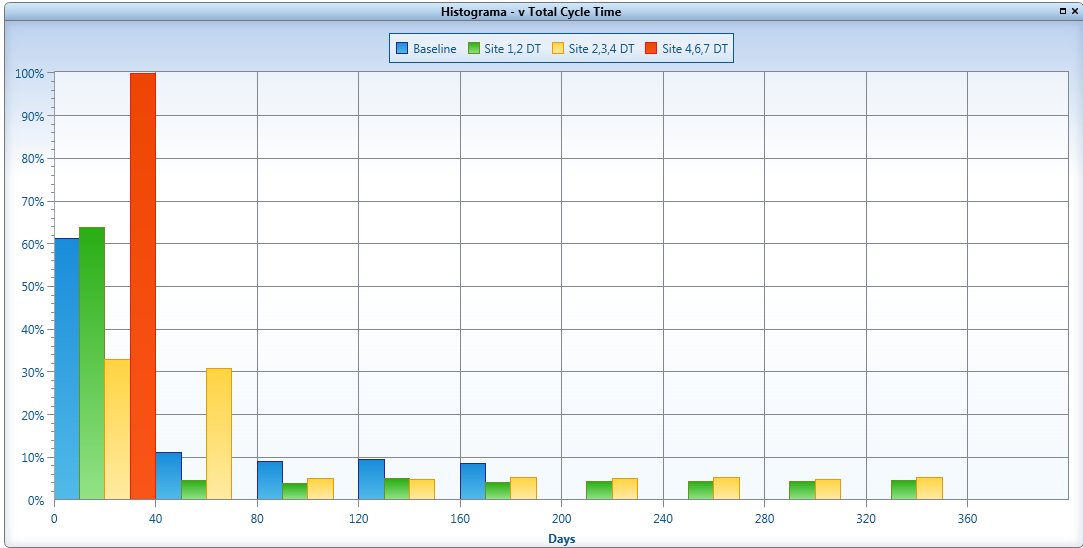
\includegraphics[width=\textwidth]{HISTOGRAMA}
	\caption{Histograma vs Ciclo Total de Tiempo}
	\label{fig:HISTOGRAMA}
\end{subfigure}
\caption{Resultados de la simulación sobre Process Simulator}\label{fig:ResultadosProcessl.}
\end{figure}

\begin{figure}[ht] 
	\centering
		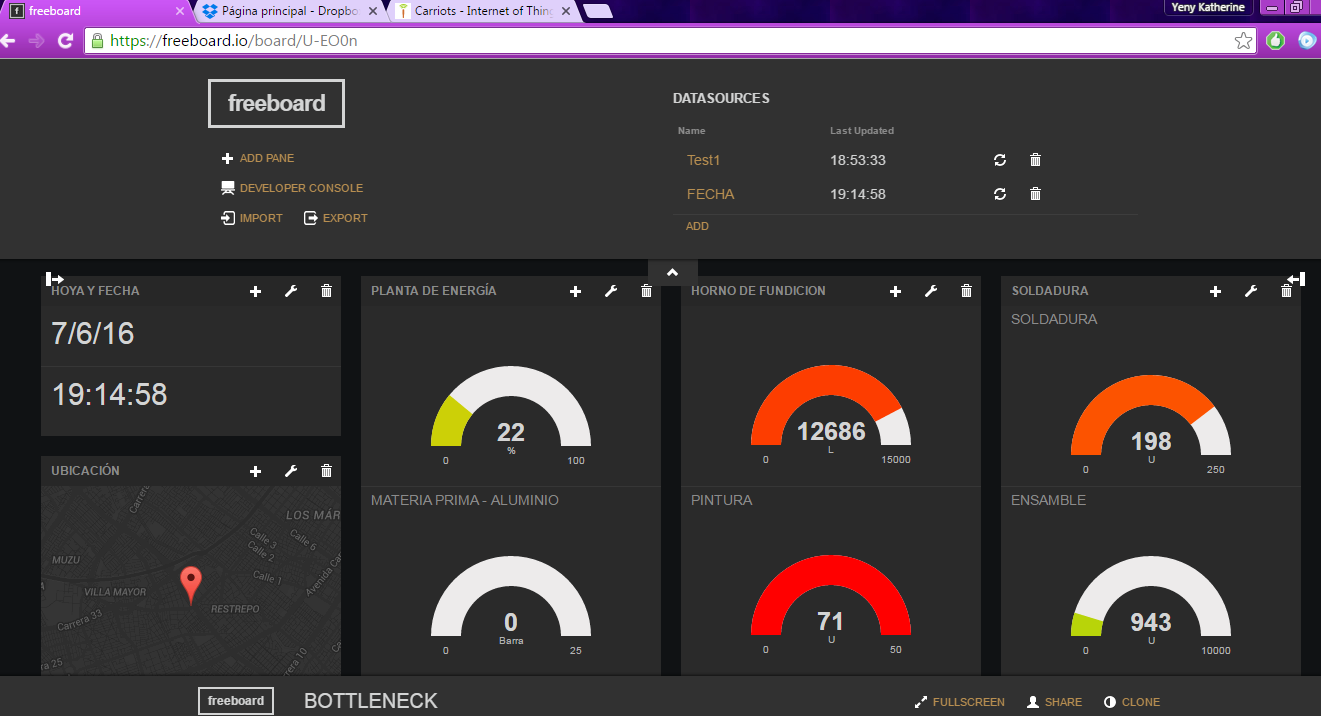
\includegraphics[scale=0.25]{RESULTADOS}   
	\caption{ \href{https://freeboard.io/board/U-EO0n}{Proceso de Producción en La Nube}} \label{fig:RESULTADOS}
\end{figure}
		
\newpage
\section{Programación Literaria dentro del informe final}

\begin{small}
\begin{lstlisting}[frame=single,style=base]	

MPW<- read.csv('"https://dl.dropbox.com/s/u5gf20h7aw8n5sr/powerplant.csv"', head = &TRUE&, col.names=c('"MUESTRA","MPW1","MPW2","MPW3","MPW4","MPW5","MPW6","MPW7","MPW8","MPW9","MPW10","MPW11"'), sep = ";")
MPW
summary(MPW)

MDL<- read.csv('"https://dl.dropbox.com/s/w79zfzj9lrnoy2q/ASSAMBLY.csv"', head = &TRUE&, col.names=c('"MUESTRA","MDL1","MDL2","MDL3","MDL4","MDL5","MDL6"'), sep = ";")
MDL
summary(MDL)

MG<- read.csv('"https://dl.dropbox.com/s/lt48p31kiumd4k5/furnace.csv"', head = &TRUE&, col.names=c('"MUESTRA","MG1","MG2","MG3","MG4","MG5","MG6","MG7","MG8","MG9"'), sep = ";")
MG
summary(MG)

ME<- read.csv('"https://dl.dropbox.com/s/ljxnb8fitqg79t4/MATERIA%20PRIMA.csv"', head = &TRUE&, col.names=c('"MUESTRA","ME1","ME2"'), sep = ";")
ME
summary(ME)

MPH<- read.csv('"https://dl.dropbox.com/s/6uvyphbse2ahtvh/PAINT.csv"', head = &TRUE&, col.names=c('"MUESTRA","MPH1","MPH2","MPH3"'), sep = ";")
MPH
summary(MPH)

MPY<- read.csv('"https://dl.dropbox.com/s/meyl8nbg5jk509g/WELDING.csv"', head = &TRUE&, col.names=c('"MUESTRA","MPY1","MPY2","MPY3","MPY4","MPY5","MPY6"'), sep = ";")
MPY
summary(MPY)

}
\end{lstlisting}
\end{small}
		
\section{Bibliografía}	
\textbf{{\Large Accesos WEB}}
	\subsection{ \href{http://cuellodebotella.com/}{Cuellos de Botella}} 
	\subsection{ \href{https://www.promodel.com/Products/ProcessSimulator}{Process Simulator 2014}} 
	\subsection{ \href{https://freeboard.io/}{Freeboard - Internet de las Cosas}} 

\bibliographystyle{apalike}						% Estilo de la bibliografía o referencias
\bibliography{biblio}							% Se muestra desde el fichero .bbl
\nocite{*}

\end{document}
